\documentclass[12pt,a4paper]{article}

% packages
  \usepackage{a4wide}
  \usepackage{tikz}

  \tikzset{st/.style = {circle, thick, minimum size=5.0mm, inner sep=0pt, draw},
           we/.style = {circle, thick, minimum size=2.0mm, inner sep=0pt, draw}}

\pagestyle{empty}

\title{Graph Algorithms and Complexity Theory - Coursework 1}
\author{Oskar Mampe}
\date{Semester 1 Session 2019--2020}

\begin{document}

\maketitle

\thispagestyle{empty}

We compute a maximum flow in this network and find a minimum cut as follows.
The left column shows the actual flow and the right column shows the residual
network with residual capacities and an augmenting path indicated by bold edges.

\begin{center}
%%%%%%%%%%%%%% ORIGINAL %%%%%%%%%%%%%%
Original Network:\\
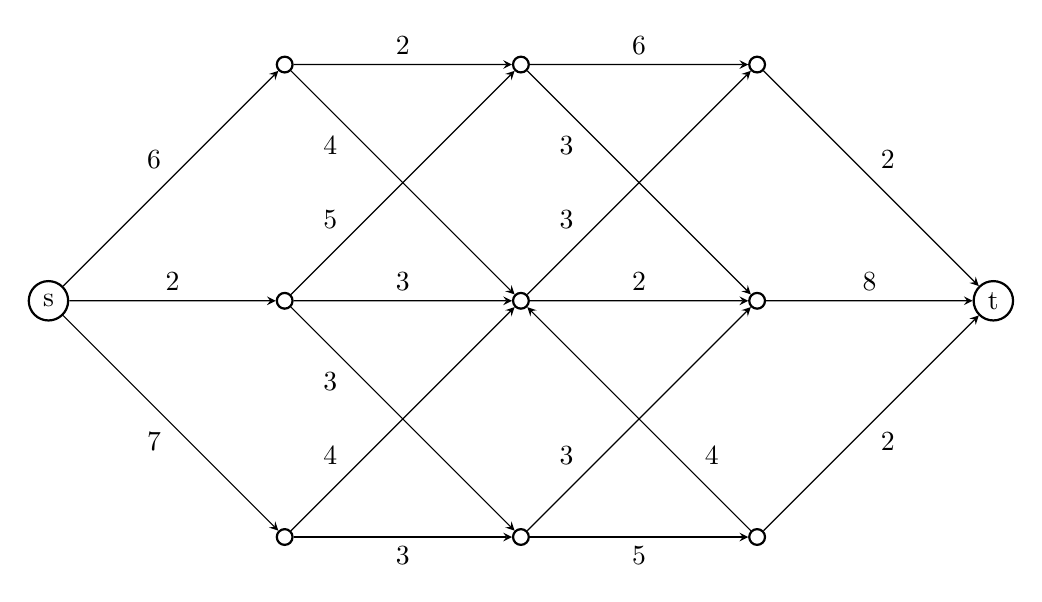
\begin{tikzpicture}[scale=1.5, >=stealth]
    \node[st] (s) at (0,2) {s};
    \node[we] (a) at (2,0) {}; \node[we] (b) at (2,2) {}; \node[we] (c) at (2,4) {}; 
    \node[we] (d) at (4,0) {}; \node[we] (e) at (4,2) {}; \node[we] (f) at (4,4) {}; 
    \node[we] (g) at (6,0) {}; \node[we] (h) at (6,2) {}; \node[we] (i) at (6,4) {}; 
    \node[st] (t) at (8,2) {t};
    \draw[->] (s) to[edge label'=7, pos=.50] (a);
    \draw[->] (s) to[edge label =2, pos=.50] (b);
    \draw[->] (s) to[edge label =6, pos=.50] (c);
    \draw[->] (a) to[edge label'=3, pos=.50] (d);
    \draw[->] (b) to[edge label =3, pos=.50] (e);
    \draw[->] (c) to[edge label =2, pos=.50] (f);
    \draw[->] (a) to[edge label =4, pos=.25] (e);
    \draw[->] (b) to[edge label =5, pos=.25] (f);
    \draw[->] (c) to[edge label'=4, pos=.25] (e);
    \draw[->] (b) to[edge label'=3, pos=.25] (d);
    \draw[->] (d) to[edge label'=5, pos=.50] (g);
    \draw[->] (e) to[edge label =2, pos=.50] (h);
    \draw[->] (f) to[edge label =6, pos=.50] (i);
    \draw[->] (d) to[edge label =3, pos=.25] (h);
    \draw[->] (e) to[edge label =3, pos=.25] (i);
    \draw[->] (f) to[edge label'=3, pos=.25] (h);
    \draw[<-] (e) to[edge label =4, pos=.75] (g);
    \draw[->] (g) to[edge label'=2, pos=.50] (t);
    \draw[->] (h) to[edge label =8, pos=.50] (t);
    \draw[->] (i) to[edge label =2, pos=.50] (t);    
  \end{tikzpicture}
  %%%%%%%%%%%%%% FIRST PASS %%%%%%%%%%%%%%
  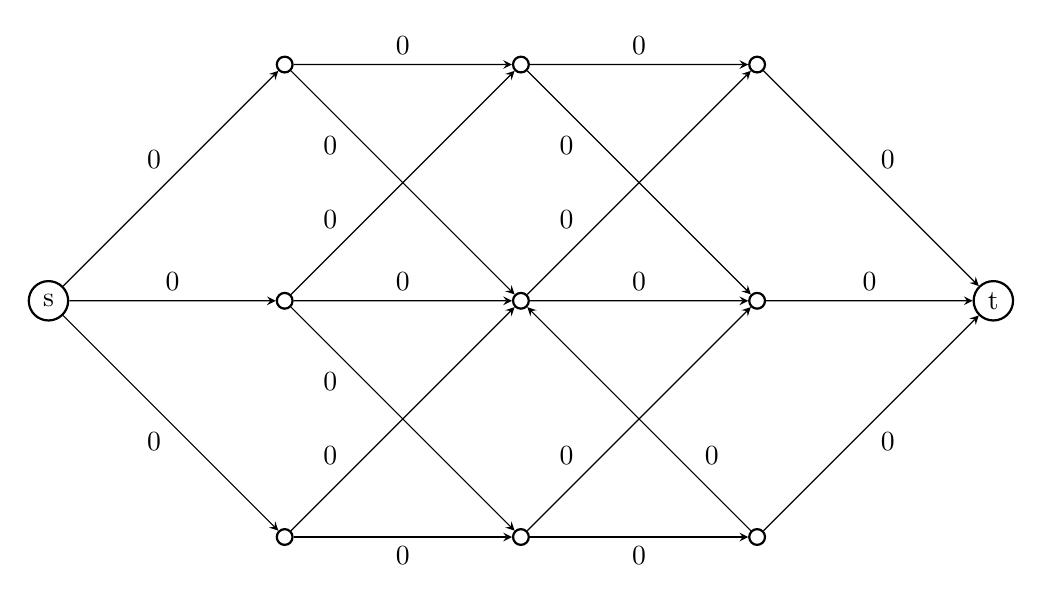
\begin{tikzpicture}[scale=1.5, >=stealth]
    \node[st] (s) at (0,2) {s};
    \node[we] (a) at (2,0) {}; \node[we] (b) at (2,2) {}; \node[we] (c) at (2,4) {}; 
    \node[we] (d) at (4,0) {}; \node[we] (e) at (4,2) {}; \node[we] (f) at (4,4) {}; 
    \node[we] (g) at (6,0) {}; \node[we] (h) at (6,2) {}; \node[we] (i) at (6,4) {}; 
    \node[st] (t) at (8,2) {t};
    \draw[->] (s) to[edge label'=0, pos=.50] (a);
    \draw[->] (s) to[edge label =0, pos=.50] (b);
    \draw[->] (s) to[edge label =0, pos=.50] (c);
    \draw[->] (a) to[edge label'=0, pos=.50] (d);
    \draw[->] (b) to[edge label =0, pos=.50] (e);
    \draw[->] (c) to[edge label =0, pos=.50] (f);
    \draw[->] (a) to[edge label =0, pos=.25] (e);
    \draw[->] (b) to[edge label =0, pos=.25] (f);
    \draw[->] (c) to[edge label'=0, pos=.25] (e);
    \draw[->] (b) to[edge label'=0, pos=.25] (d);
    \draw[->] (d) to[edge label'=0, pos=.50] (g);
    \draw[->] (e) to[edge label =0, pos=.50] (h);
    \draw[->] (f) to[edge label =0, pos=.50] (i);
    \draw[->] (d) to[edge label =0, pos=.25] (h);
    \draw[->] (e) to[edge label =0, pos=.25] (i);
    \draw[->] (f) to[edge label'=0, pos=.25] (h);
    \draw[<-] (e) to[edge label =0, pos=.75] (g);
    \draw[->] (g) to[edge label'=0, pos=.50] (t);
    \draw[->] (h) to[edge label =0, pos=.50] (t);
    \draw[->] (i) to[edge label =0, pos=.50] (t);    
  \end{tikzpicture}
    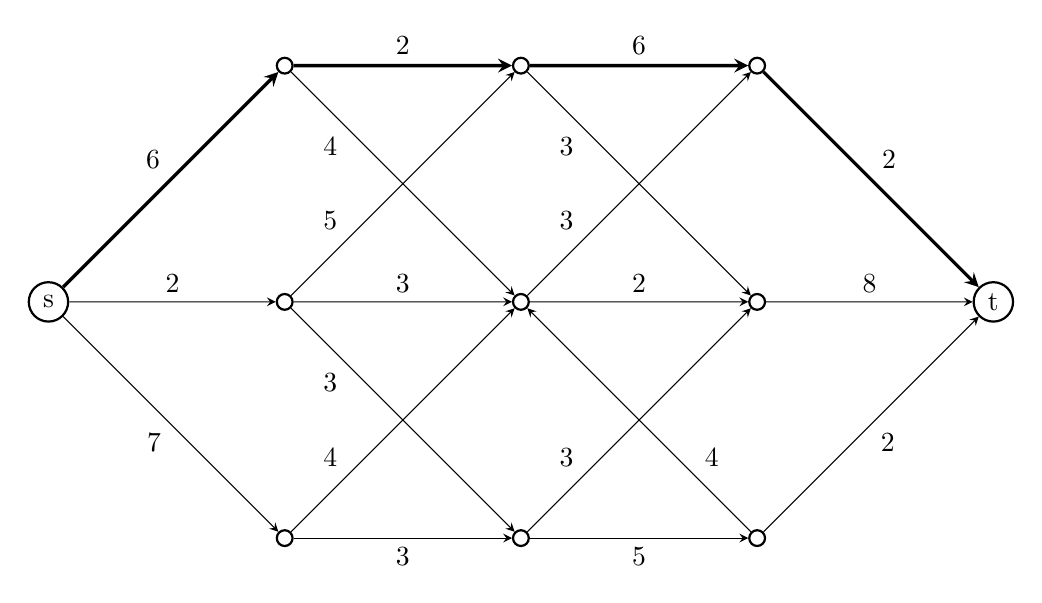
\begin{tikzpicture}[scale=1.5, >=stealth]
    \node[st] (s) at (0,2) {s};
    \node[we] (a) at (2,0) {}; \node[we] (b) at (2,2) {}; \node[we] (c) at (2,4) {}; 
    \node[we] (d) at (4,0) {}; \node[we] (e) at (4,2) {}; \node[we] (f) at (4,4) {}; 
    \node[we] (g) at (6,0) {}; \node[we] (h) at (6,2) {}; \node[we] (i) at (6,4) {}; 
    \node[st] (t) at (8,2) {t};
    \draw[->] (s) to[edge label'=7, pos=.50] (a);
    \draw[->] (s) to[edge label =2, pos=.50] (b);
    \draw[->, very thick] (s) to[edge label =6, pos=.50] (c);
    \draw[->] (a) to[edge label'=3, pos=.50] (d);
    \draw[->] (b) to[edge label =3, pos=.50] (e);
    \draw[->, very thick] (c) to[edge label =2, pos=.50] (f);
    \draw[->] (a) to[edge label =4, pos=.25] (e);
    \draw[->] (b) to[edge label =5, pos=.25] (f);
    \draw[->] (c) to[edge label'=4, pos=.25] (e);
    \draw[->] (b) to[edge label'=3, pos=.25] (d);
    \draw[->] (d) to[edge label'=5, pos=.50] (g);
    \draw[->] (e) to[edge label =2, pos=.50] (h);
    \draw[->, very thick] (f) to[edge label =6, pos=.50] (i);
    \draw[->] (d) to[edge label =3, pos=.25] (h);
    \draw[->] (e) to[edge label =3, pos=.25] (i);
    \draw[->] (f) to[edge label'=3, pos=.25] (h);
    \draw[<-] (e) to[edge label =4, pos=.75] (g);
    \draw[->] (g) to[edge label'=2, pos=.50] (t);
    \draw[->] (h) to[edge label =8, pos=.50] (t);
    \draw[->, very thick] (i) to[edge label =2, pos=.50] (t);    
  \end{tikzpicture}
  
  %%%%%%%%%%%%%% SECOND PASS %%%%%%%%%%%%%%
   
    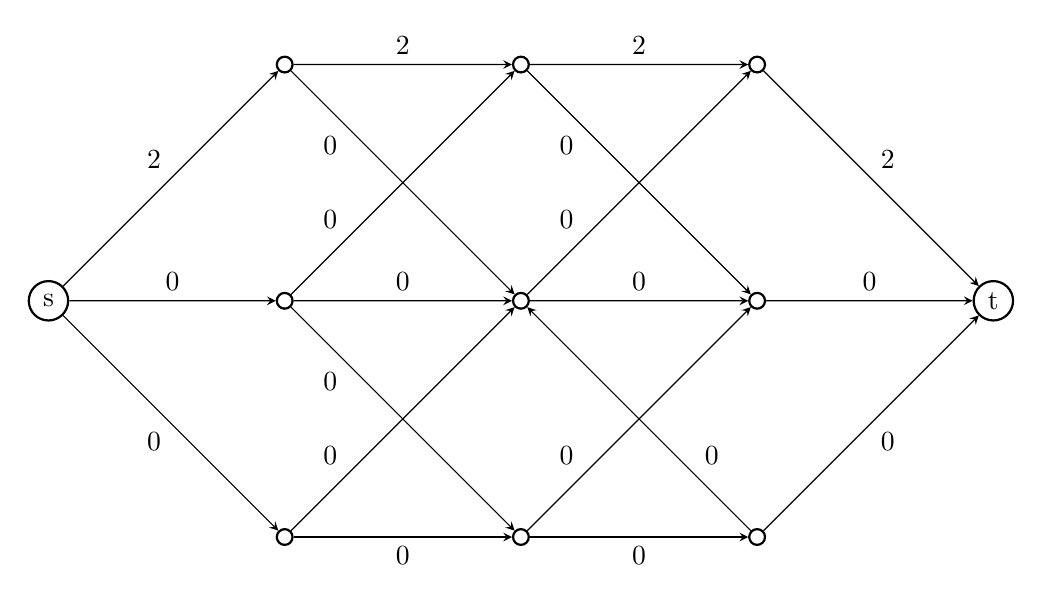
\begin{tikzpicture}[scale=1.5, >=stealth]
    \node[st] (s) at (0,2) {s};
    \node[we] (a) at (2,0) {}; \node[we] (b) at (2,2) {}; \node[we] (c) at (2,4) {}; 
    \node[we] (d) at (4,0) {}; \node[we] (e) at (4,2) {}; \node[we] (f) at (4,4) {}; 
    \node[we] (g) at (6,0) {}; \node[we] (h) at (6,2) {}; \node[we] (i) at (6,4) {}; 
    \node[st] (t) at (8,2) {t};
    \draw[->] (s) to[edge label'=0, pos=.50] (a);
    \draw[->] (s) to[edge label =0, pos=.50] (b);
    \draw[->] (s) to[edge label =2, pos=.50] (c);
    \draw[->] (a) to[edge label'=0, pos=.50] (d);
    \draw[->] (b) to[edge label =0, pos=.50] (e);
    \draw[->] (c) to[edge label =2, pos=.50] (f);
    \draw[->] (a) to[edge label =0, pos=.25] (e);
    \draw[->] (b) to[edge label =0, pos=.25] (f);
    \draw[->] (c) to[edge label'=0, pos=.25] (e);
    \draw[->] (b) to[edge label'=0, pos=.25] (d);
    \draw[->] (d) to[edge label'=0, pos=.50] (g);
    \draw[->] (e) to[edge label =0, pos=.50] (h);
    \draw[->] (f) to[edge label =2, pos=.50] (i);
    \draw[->] (d) to[edge label =0, pos=.25] (h);
    \draw[->] (e) to[edge label =0, pos=.25] (i);
    \draw[->] (f) to[edge label'=0, pos=.25] (h);
    \draw[<-] (e) to[edge label =0, pos=.75] (g);
    \draw[->] (g) to[edge label'=0, pos=.50] (t);
    \draw[->] (h) to[edge label =0, pos=.50] (t);
    \draw[->] (i) to[edge label =2, pos=.50] (t);    
  \end{tikzpicture}
    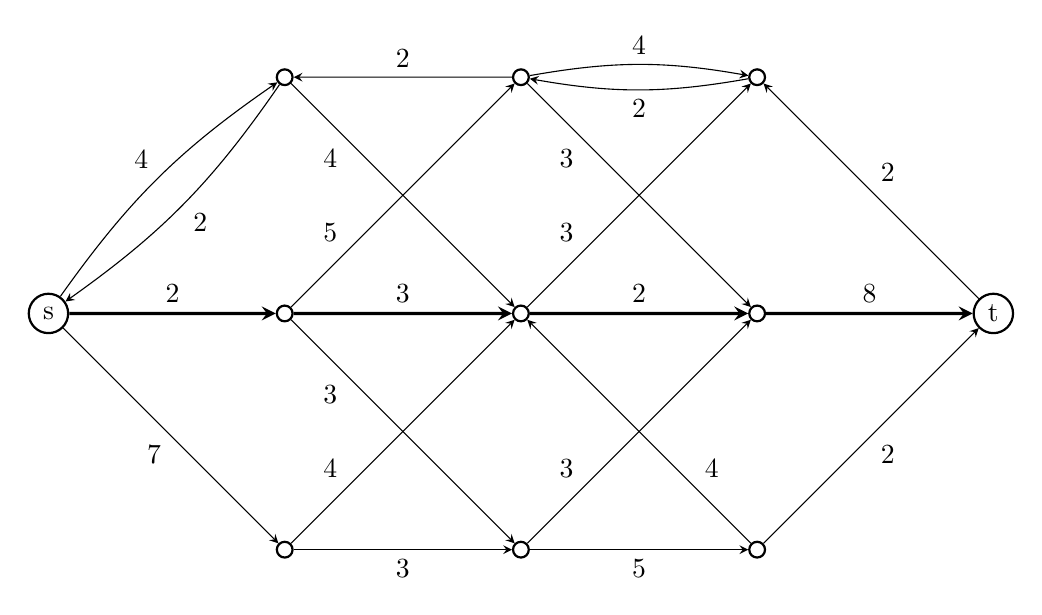
\begin{tikzpicture}[scale=1.5, >=stealth, bend angle=10]
    \node[st] (s) at (0,2) {s};
    \node[we] (a) at (2,0) {}; \node[we] (b) at (2,2) {}; \node[we] (c) at (2,4) {}; 
    \node[we] (d) at (4,0) {}; \node[we] (e) at (4,2) {}; \node[we] (f) at (4,4) {}; 
    \node[we] (g) at (6,0) {}; \node[we] (h) at (6,2) {}; \node[we] (i) at (6,4) {}; 
    \node[st] (t) at (8,2) {t};
    \draw[->] (s) to[edge label'=7, pos=.50] (a);
    \draw[->, very thick] (s) to[edge label =2, pos=.50] (b);
    \draw[->] (s) to[bend left, edge label =4, pos=.50] (c);
    \draw[<-] (s) to[bend right, edge label'=2, pos=.50] (c);
    \draw[->] (a) to[edge label'=3, pos=.50] (d);
    \draw[->, very thick] (b) to[edge label =3, pos=.50] (e);
    \draw[<-] (c) to[edge label =2, pos=.50] (f);
    \draw[->] (a) to[edge label =4, pos=.25] (e);
    \draw[->] (b) to[edge label =5, pos=.25] (f);
    \draw[->] (c) to[edge label'=4, pos=.25] (e);
    \draw[->] (b) to[edge label'=3, pos=.25] (d);
    \draw[->] (d) to[edge label'=5, pos=.50] (g);
    \draw[->, very thick] (e) to[edge label =2, pos=.50] (h);
    \draw[->] (f) to[bend left, edge label =4, pos=.50] (i);
    \draw[<-] (f) to[bend right, edge label'=2, pos=.50] (i);
    \draw[->] (d) to[edge label =3, pos=.25] (h);
    \draw[->] (e) to[edge label =3, pos=.25] (i);
    \draw[->] (f) to[edge label'=3, pos=.25] (h);
    \draw[<-] (e) to[edge label =4, pos=.75] (g);
    \draw[->] (g) to[edge label'=2, pos=.50] (t);
    \draw[->, very thick] (h) to[edge label =8, pos=.50] (t);
    \draw[<-] (i) to[edge label =2, pos=.50] (t);    
  \end{tikzpicture}
  
  %%%%%%%%%%%%%% THIRD PASS %%%%%%%%%%%%%%

 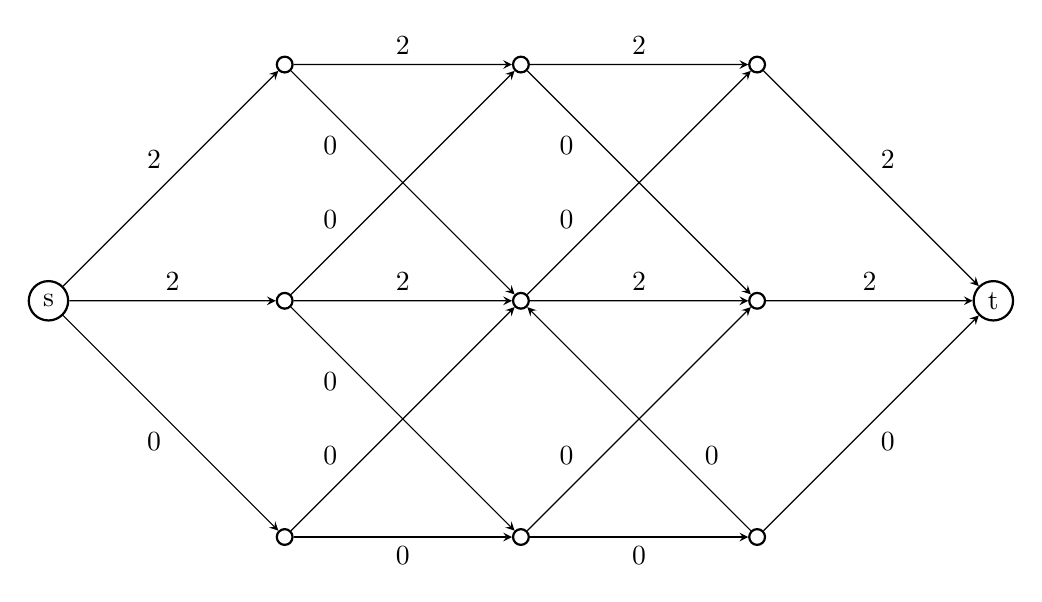
\begin{tikzpicture}[scale=1.5, >=stealth]
    \node[st] (s) at (0,2) {s};
    \node[we] (a) at (2,0) {}; \node[we] (b) at (2,2) {}; \node[we] (c) at (2,4) {}; 
    \node[we] (d) at (4,0) {}; \node[we] (e) at (4,2) {}; \node[we] (f) at (4,4) {}; 
    \node[we] (g) at (6,0) {}; \node[we] (h) at (6,2) {}; \node[we] (i) at (6,4) {}; 
    \node[st] (t) at (8,2) {t};
    \draw[->] (s) to[edge label'=0, pos=.50] (a);
    \draw[->] (s) to[edge label =2, pos=.50] (b);
    \draw[->] (s) to[edge label =2, pos=.50] (c);
    \draw[->] (a) to[edge label'=0, pos=.50] (d);
    \draw[->] (b) to[edge label =2, pos=.50] (e);
    \draw[->] (c) to[edge label =2, pos=.50] (f);
    \draw[->] (a) to[edge label =0, pos=.25] (e);
    \draw[->] (b) to[edge label =0, pos=.25] (f);
    \draw[->] (c) to[edge label'=0, pos=.25] (e);
    \draw[->] (b) to[edge label'=0, pos=.25] (d);
    \draw[->] (d) to[edge label'=0, pos=.50] (g);
    \draw[->] (e) to[edge label =2, pos=.50] (h);
    \draw[->] (f) to[edge label =2, pos=.50] (i);
    \draw[->] (d) to[edge label =0, pos=.25] (h);
    \draw[->] (e) to[edge label =0, pos=.25] (i);
    \draw[->] (f) to[edge label'=0, pos=.25] (h);
    \draw[<-] (e) to[edge label =0, pos=.75] (g);
    \draw[->] (g) to[edge label'=0, pos=.50] (t);
    \draw[->] (h) to[edge label =2, pos=.50] (t);
    \draw[->] (i) to[edge label =2, pos=.50] (t);    
  \end{tikzpicture}
    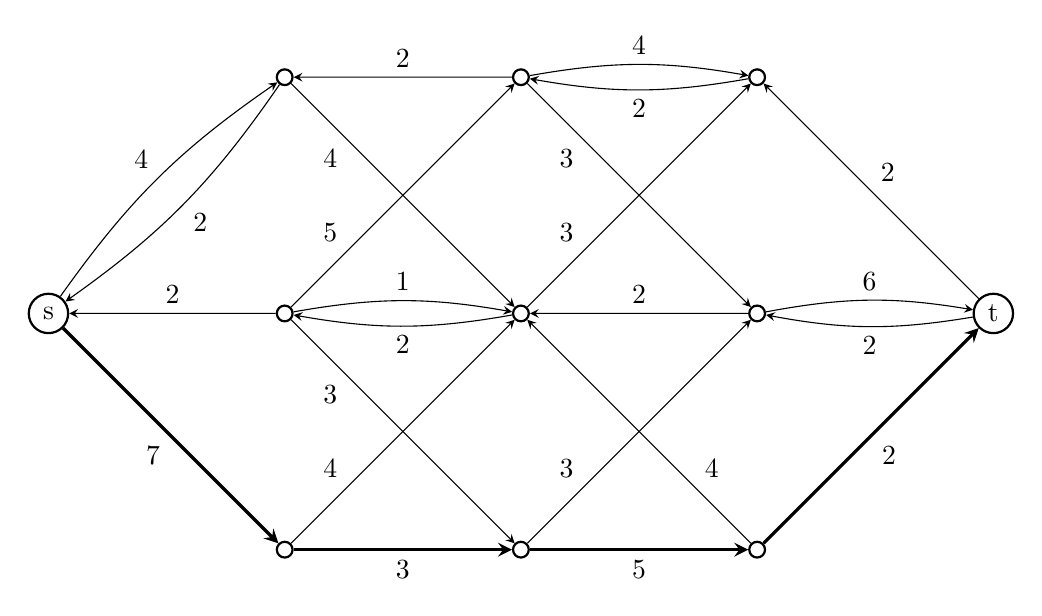
\begin{tikzpicture}[scale=1.5, >=stealth, bend angle=10]
    \node[st] (s) at (0,2) {s};
    \node[we] (a) at (2,0) {}; \node[we] (b) at (2,2) {}; \node[we] (c) at (2,4) {}; 
    \node[we] (d) at (4,0) {}; \node[we] (e) at (4,2) {}; \node[we] (f) at (4,4) {}; 
    \node[we] (g) at (6,0) {}; \node[we] (h) at (6,2) {}; \node[we] (i) at (6,4) {}; 
    \node[st] (t) at (8,2) {t};
    \draw[->, very thick] (s) to[edge label'=7, pos=.50] (a);
    \draw[<-] (s) to[edge label =2, pos=.50] (b);
    \draw[->] (s) to[bend left, edge label =4, pos=.50] (c);
    \draw[<-] (s) to[bend right, edge label'=2, pos=.50] (c);
    \draw[->, very thick] (a) to[edge label'=3, pos=.50] (d);
    \draw[->] (b) to[bend left, edge label =1, pos=.50] (e);
    \draw[<-] (b) to[bend right, edge label'=2, pos=.50] (e);
    \draw[<-] (c) to[edge label =2, pos=.50] (f);
    \draw[->] (a) to[edge label =4, pos=.25] (e);
    \draw[->] (b) to[edge label =5, pos=.25] (f);
    \draw[->] (c) to[edge label'=4, pos=.25] (e);
    \draw[->] (b) to[edge label'=3, pos=.25] (d);
    \draw[->,very thick] (d) to[edge label'=5, pos=.50] (g);
    \draw[<-] (e) to[edge label =2, pos=.50] (h);
    \draw[->] (f) to[bend left, edge label =4, pos=.50] (i);
    \draw[<-] (f) to[bend right, edge label'=2, pos=.50] (i);
    \draw[->] (d) to[edge label =3, pos=.25] (h);
    \draw[->] (e) to[edge label =3, pos=.25] (i);
    \draw[->] (f) to[edge label'=3, pos=.25] (h);
    \draw[<-] (e) to[edge label =4, pos=.75] (g);
    \draw[->, very thick] (g) to[edge label'=2, pos=.50] (t);
    \draw[->] (h) to[bend left, edge label =6, pos=.50] (t);
    \draw[<-] (h) to[bend right, edge label'=2, pos=.50] (t);
    \draw[<-] (i) to[edge label =2, pos=.50] (t);   
  \end{tikzpicture}
  
  %%%%%%%%%%%%%% FOURTH PASS %%%%%%%%%%%%%%

 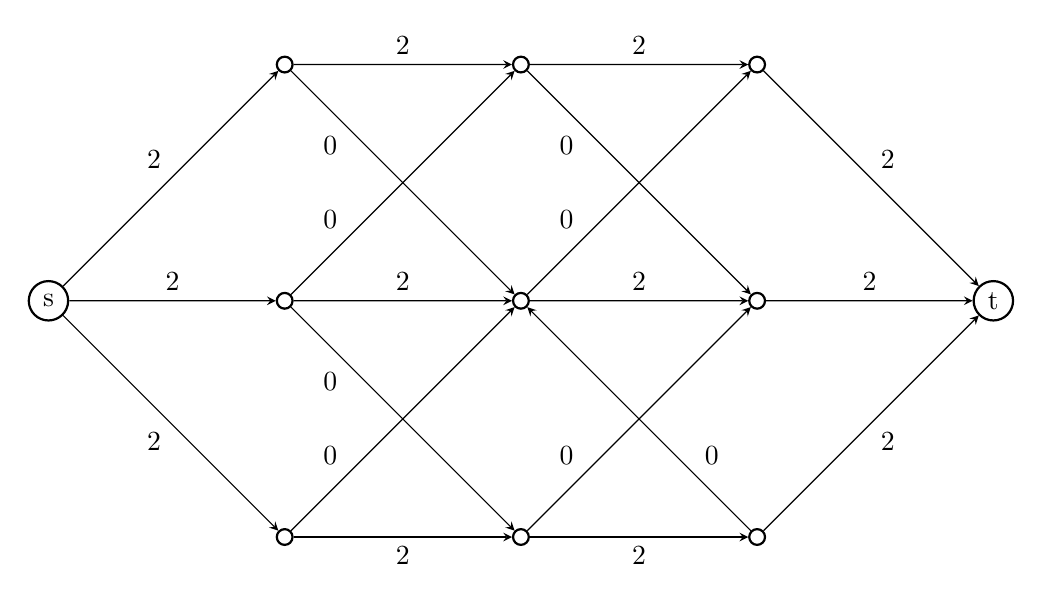
\begin{tikzpicture}[scale=1.5, >=stealth]
    \node[st] (s) at (0,2) {s};
    \node[we] (a) at (2,0) {}; \node[we] (b) at (2,2) {}; \node[we] (c) at (2,4) {}; 
    \node[we] (d) at (4,0) {}; \node[we] (e) at (4,2) {}; \node[we] (f) at (4,4) {}; 
    \node[we] (g) at (6,0) {}; \node[we] (h) at (6,2) {}; \node[we] (i) at (6,4) {}; 
    \node[st] (t) at (8,2) {t};
    \draw[->] (s) to[edge label'=2, pos=.50] (a);
    \draw[->] (s) to[edge label =2, pos=.50] (b);
    \draw[->] (s) to[edge label =2, pos=.50] (c);
    \draw[->] (a) to[edge label'=2, pos=.50] (d);
    \draw[->] (b) to[edge label =2, pos=.50] (e);
    \draw[->] (c) to[edge label =2, pos=.50] (f);
    \draw[->] (a) to[edge label =0, pos=.25] (e);
    \draw[->] (b) to[edge label =0, pos=.25] (f);
    \draw[->] (c) to[edge label'=0, pos=.25] (e);
    \draw[->] (b) to[edge label'=0, pos=.25] (d);
    \draw[->] (d) to[edge label'=2, pos=.50] (g);
    \draw[->] (e) to[edge label =2, pos=.50] (h);
    \draw[->] (f) to[edge label =2, pos=.50] (i);
    \draw[->] (d) to[edge label =0, pos=.25] (h);
    \draw[->] (e) to[edge label =0, pos=.25] (i);
    \draw[->] (f) to[edge label'=0, pos=.25] (h);
    \draw[<-] (e) to[edge label =0, pos=.75] (g);
    \draw[->] (g) to[edge label'=2, pos=.50] (t);
    \draw[->] (h) to[edge label =2, pos=.50] (t);
    \draw[->] (i) to[edge label =2, pos=.50] (t);    
  \end{tikzpicture}
    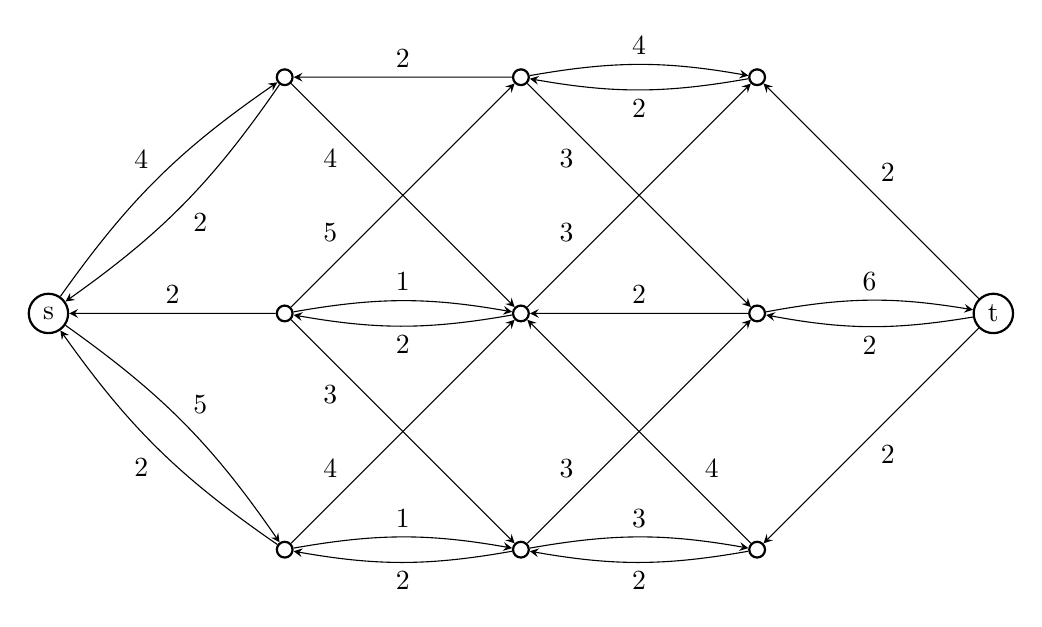
\begin{tikzpicture}[scale=1.5, >=stealth, bend angle=10]
    \node[st] (s) at (0,2) {s};
    \node[we] (a) at (2,0) {}; \node[we] (b) at (2,2) {}; \node[we] (c) at (2,4) {}; 
    \node[we] (d) at (4,0) {}; \node[we] (e) at (4,2) {}; \node[we] (f) at (4,4) {}; 
    \node[we] (g) at (6,0) {}; \node[we] (h) at (6,2) {}; \node[we] (i) at (6,4) {}; 
    \node[st] (t) at (8,2) {t};
    \draw[->] (s) to[bend left, edge label=5, pos=.50] (a);
    \draw[<-] (s) to[bend right, edge label'=2, pos=.50] (a);
    \draw[<-] (s) to[edge label =2, pos=.50] (b);
    \draw[->] (s) to[bend left, edge label =4, pos=.50] (c);
    \draw[<-] (s) to[bend right, edge label'=2, pos=.50] (c);
    \draw[->] (a) to[bend left, edge label=1, pos=.50] (d);
    \draw[<-] (a) to[bend right, edge label'=2, pos=.50] (d);
    \draw[->] (b) to[bend left, edge label =1, pos=.50] (e);
    \draw[<-] (b) to[bend right, edge label'=2, pos=.50] (e);
    \draw[<-] (c) to[edge label =2, pos=.50] (f);
    \draw[->] (a) to[edge label =4, pos=.25] (e);
    \draw[->] (b) to[edge label =5, pos=.25] (f);
    \draw[->] (c) to[edge label'=4, pos=.25] (e);
    \draw[->] (b) to[edge label'=3, pos=.25] (d);
    \draw[->] (d) to[bend left, edge label=3, pos=.50] (g);
    \draw[<-] (d) to[bend right, edge label'=2, pos=.50] (g);
    \draw[<-] (e) to[edge label =2, pos=.50] (h);
    \draw[->] (f) to[bend left, edge label =4, pos=.50] (i);
    \draw[<-] (f) to[bend right, edge label'=2, pos=.50] (i);
    \draw[->] (d) to[edge label =3, pos=.25] (h);
    \draw[->] (e) to[edge label =3, pos=.25] (i);
    \draw[->] (f) to[edge label'=3, pos=.25] (h);
    \draw[<-] (e) to[edge label =4, pos=.75] (g);
    \draw[<-] (g) to[edge label'=2, pos=.50] (t);
    \draw[->] (h) to[bend left, edge label =6, pos=.50] (t);
    \draw[<-] (h) to[bend right, edge label'=2, pos=.50] (t);
    \draw[<-] (i) to[edge label =2, pos=.50] (t);   
  \end{tikzpicture}
\end{center}

\vspace{\fill}

The last flow has value 12. A cut $(A,B)$ of this capacity is defined
by square white vertices in $A$ and round black vertices in $B$. 
Therefore the flow is maximum and the cut $(A,B)$ is a minimum cut.
The edges across the cut $(A,B)$ are indicated by dashed lines.

\end{document}
